
To evaluate the reproducibility of our results, we conducted three experiments to examine the uncertainties related to\\
\\
\textbf{A} manually positioning the fibres between measurements, \\
\textbf{B} recalibrating the polarisation crystal between measurements, \\
\textbf{C} recording transmission through a fabricated design after resetting both the fiber positions and polarisation. For all of these three experiments, the supercontinuum laser was used as a light source (see Table \ref{tablelightsources}).\\
\\
In \textbf{A}, we recorded the transmission through a reference waveguide. \\
In \textbf{B}, we recorded the transmission through a photonic crystal with a cut-off at $\approx$ 1560 nm.\\
In \textbf{C}, we recorded the transmission through a fabricated box structure with feature size 40 nm.

\subsection{Fiber positioning}

For every measurement recorded, the optical fibres must be positioned in order to get a signal through the current silicon structures. This contributes an uncertainty when normalising the signal from the designed structure with the reference waveguide. Five sets of measurements were performed with the supercontinuum laser on a reference waveguide. The supercontinuum has an intensity profile as seen in the appendix Fig. \ref{fig:superKref}. 
For each 5 data points at a given wavelength, the standard deviation of transmission is computed. As seen on Fig. \ref{fig:PositionError}, the standard deviations are on average 0.3 dB, and the highest deviation is around 1.2 dB. 

\begin{figure}[h!]
    \centering
    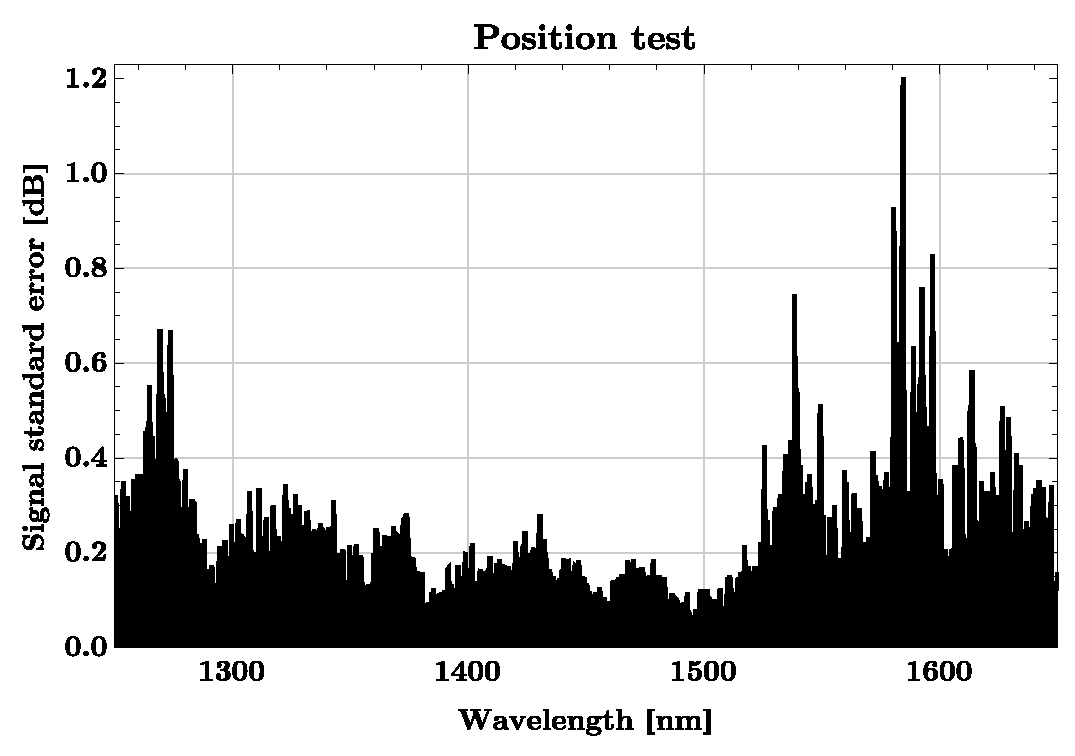
\includegraphics[width=0.8\textwidth]{fig/statistics/positiontest.eps}
    \caption{Standard deviation vs wavelength from positioning fibres.}
    \label{fig:PositionError}
\end{figure}

\subsection{Polarisation}

The intensity is highly dependent on the orientation of the twisters, so several measurements were gathered with the orientation of the twisters scrambled and then repositioned/optimised before each individual measurement. The results are shown in Fig. \ref{fig:PolarisationError}. \\

\begin{figure}[h!]
    \centering  
    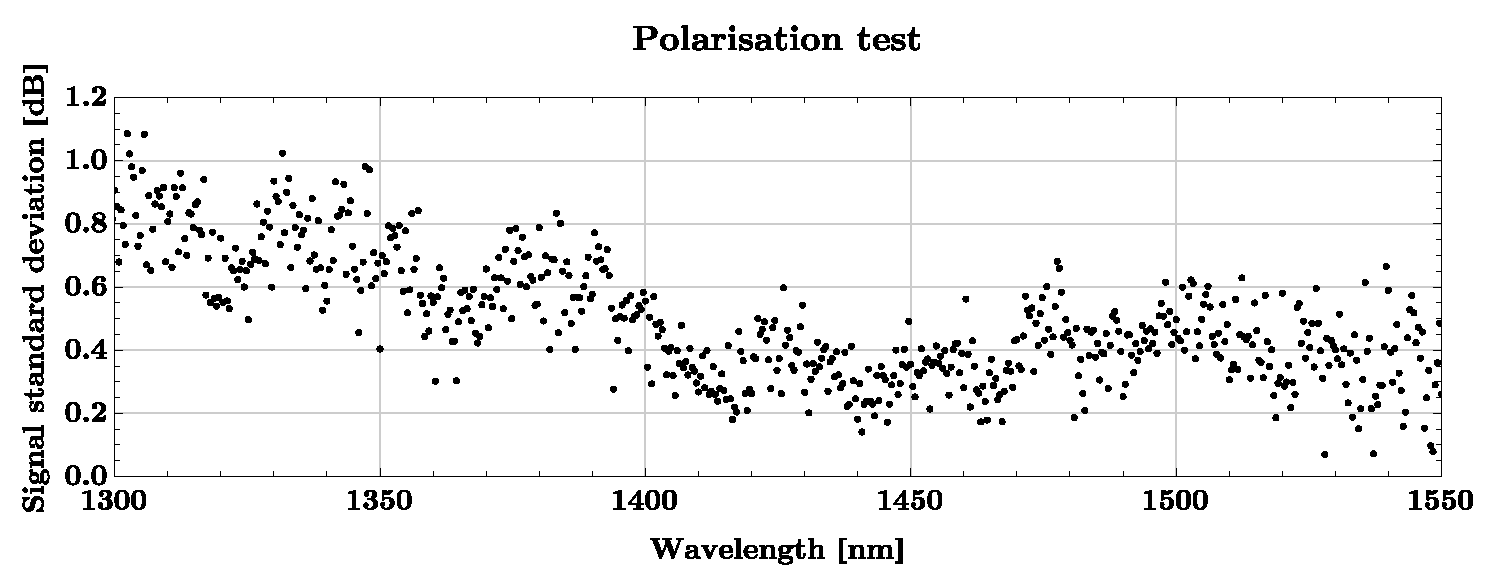
\includegraphics[width=\textwidth]{fig/statistics/polarisationtest2.eps}
    \caption{Standard deviation vs wavelength from setting polarisation with twisters.}
    \label{fig:PolarisationError}
\end{figure}

The measurements cover wavelengths below 1560 nm, since the photonic crystal cuts of higher wavelengths.

In Fig. \ref{fig:PolarisationError} we look at a section of the spectrum which is not dominated by background noise. We see that the standard deviation is no more than 2.0 dB, which suggests that the polarisation deviation is not the cause of the drastic fluctuations at wavelengths from the upper output waveguide within [1400, 1600] nm on Fig. \ref{fig:transmissionkilde3}.

\subsection{Consecutive readings of a single design}

The positions of the fibres and polarisation seem not to be the main cause of the observed fluctuations. As a final statistical analysis, we compute standard deviations from five sets of normalised data of the 40 nm box-formed design. Thus, five times we measured the signal through the design and reference waveguide.  Between each measurement set (of reference and design), the polarisation and position were scrambled and reset. Signal measurements can be seen in appendix Fig. \ref{fig:ConsecutiveFiveBox40}.

\begin{figure}[h!]
    \centering
    \begin{subfigure}[h!]{0.8\textwidth}
    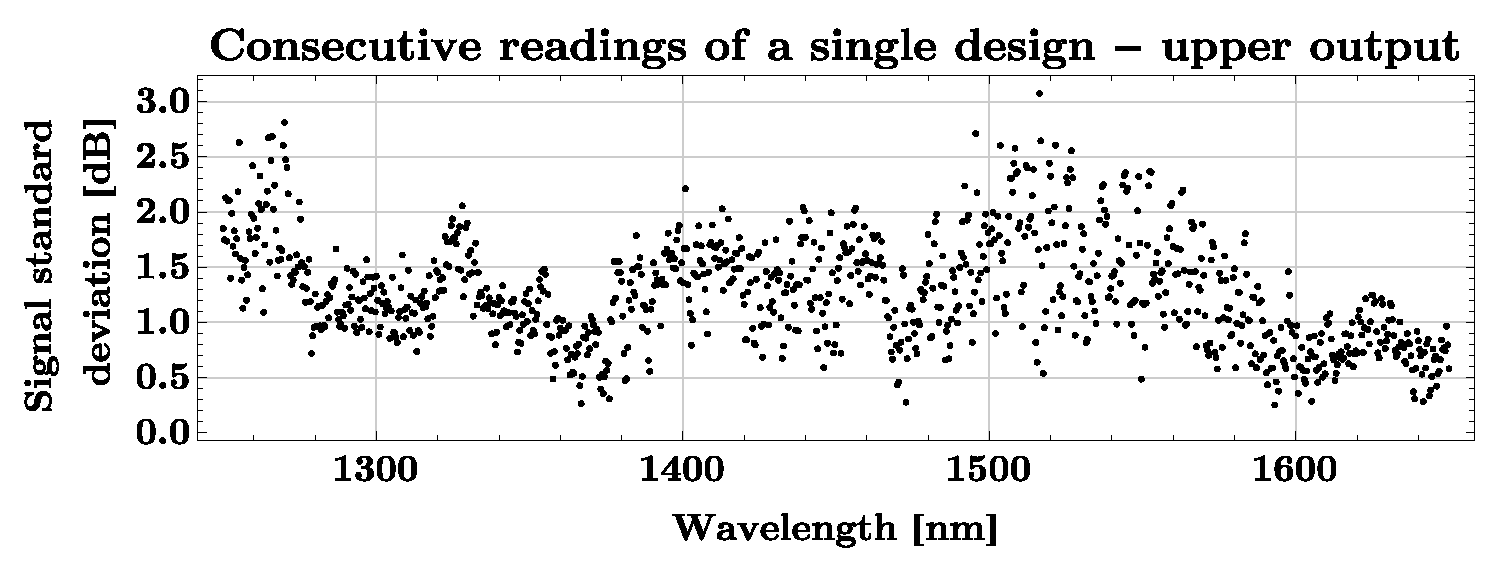
\includegraphics[width=\textwidth]{fig/statistics/ReproducibilityTestUpper.eps}
    \caption{Signal standard deviation in the upper output waveguide. This channel is intended to deliver light peaking at wavelength 1300 nm.}
    \label{fig:RepNorm1}
    \end{subfigure}

     \begin{subfigure}[h!]{0.8\textwidth}
    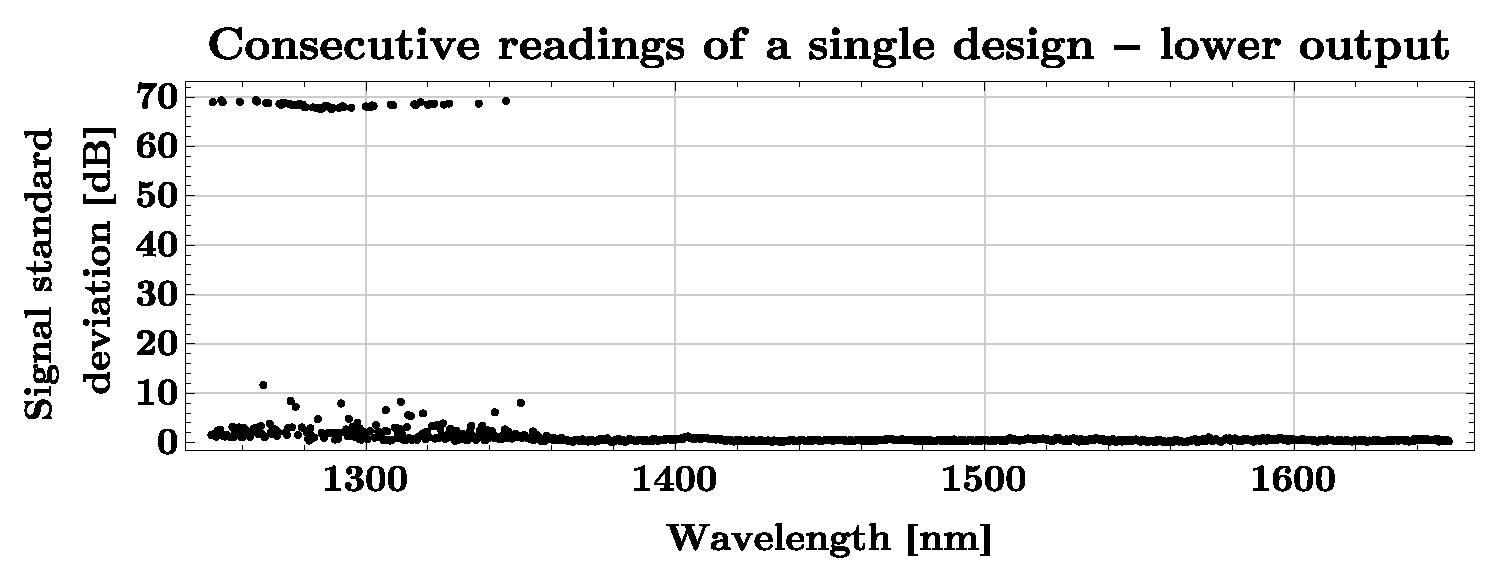
\includegraphics[width=\textwidth]{fig/statistics/ReproducibilityTestLower1250.eps}
    \caption{Signal standard deviation in the lower output waveguide. This channel is intended to deliver light peaking at wavelength 1550 nm.}
    \label{fig:RepNorm2}
    \end{subfigure}

     \begin{subfigure}[h!]{0.8\textwidth}
    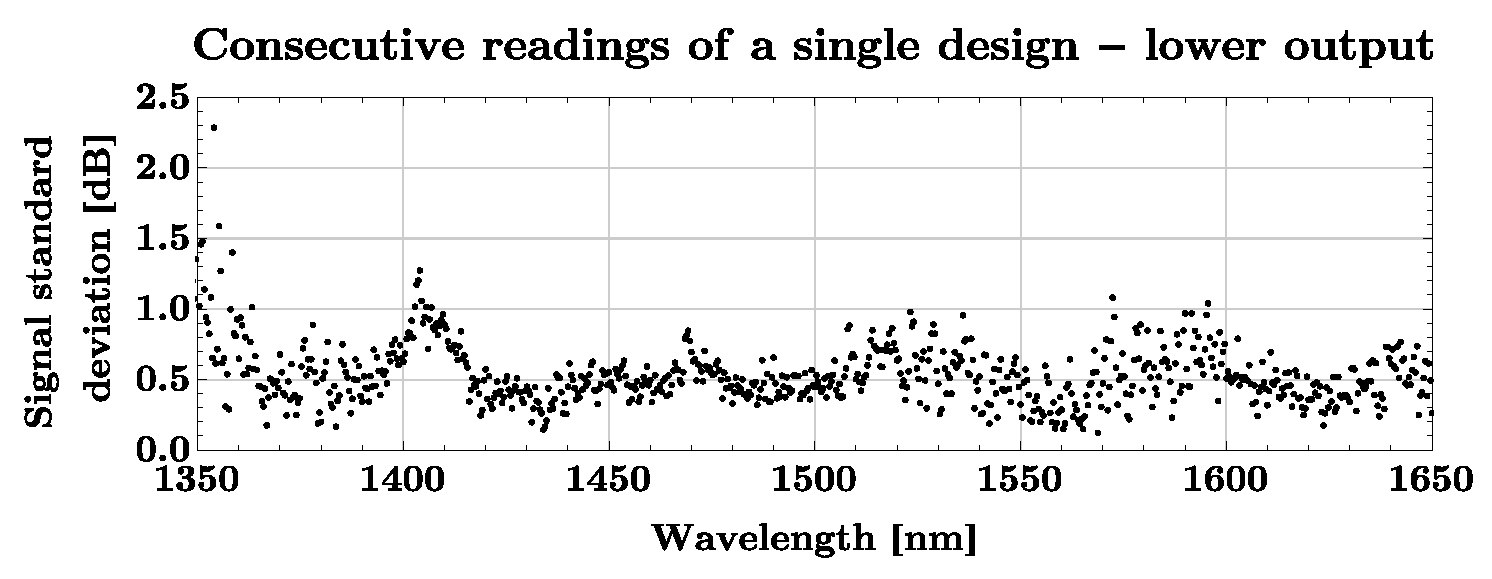
\includegraphics[width=\textwidth]{fig/statistics/ReproducibilityTestLower1350.eps}
    \caption{Section of the spectrum from Fig. \ref{fig:RepNorm2} not being dominated by background noise.}
    \label{fig:RepNorm3}
    \end{subfigure}
    
    \caption{Standard deviation vs wavelength of data from several measurements of the same structure.}
    \label{fig:RepNorm}
\end{figure}

From the measured data on Fig. \ref{fig:RepNorm1}, we read an average standard deviation around 1.5 dB and a maximum deviation around 3.1 dB for the signal through the upper waveguide. From the measured data on Fig. \ref{fig:RepNorm2} concerning the lower output waveguide, the maximum standard deviation is a whopping 70 dB. (This aberration is discussed in the next section.) If we look at the section without this disturbance on Fig. \ref{fig:RepNorm3} we see a standard deviation below 2.5 dB. 

\subsection{Analysis and discussion} 

From repositioning the fibres, the uncertainty (standard deviation) is on average 0.3 dB and at most 1.2 dB. From adjusting the polarisation, the standard deviation is on average 0.5 dB and at most 1.1 dB. \\
As these uncertainties should be independent (since we did not reposition the fibres during the polarisation test and vice versa), we calculate the combined uncertainty by adding the variances (that is, the squares of the standard deviations) and taking the square root. Thus we should expect the combined uncertainty to be on average 0.6 dB and 1.6 dB at most.\\ \vspace{1cm}

Looking at the statistical analysis of the lower waveguide  (Fig. \ref{fig:RepNorm3}), the uncertainty looks pretty much on the mark. The huge amount of noise at the low wavelengths (see Fig. \ref{fig:RepNorm2}) is caused by a single data sample, see Fig. \ref{fig:ConsecutiveFiveBox40} in Appendix. This sample has a signal intensity below the sensitivity of the OSA and can therefore be ignored. So it appears that repositioning the fibres and setting the polarisation are the main contributors to the uncertainty. 
\\
However, looking at the upper waveguide (Fig. \ref{fig:RepNorm1}) the deviations are much higher, on average 1.5 dB and peaking at 3.1 dB. This is actually on par with the large uncertainties on the upper waveguide in Fig. \ref{fig:transmissionkilde3_a} estimated by 5-blocking the data. (Note that the shaded regions mark maximum and minimum values. The distance from the average to a maximum or minimum value should be roughly two standard deviations.)\\

The change in uncertainty may be explained by the fact that the upper waveguide covers more low-intensity signal. Since the intensity of background noise is absolute, it should have a stronger relative influence on lower intensities. \\

%%%%%%%%%%%%%%%%%%Furthermore, the lower wavelengths have a higher dependency on the minimum feature size of the structure, meaning the binary division of shaded areas to either black or white effects the lower end of the spectrum more. \\ 

In summary, we estimate that the experimental results are reproducible within a margin of error (standard deviation) of 1.6 dB when looking at signal with high transmission, while the crosstalk-results are reproducible within a margin of error (standard deviation) of 3.1 dB. These estimates are quite pessimistic, but it is necessary when it is taken into account that the measurements are based on one of the structures. In order to lower the uncertainties, more experiments would have to be conducted.

